%%%%%%%%%%%%%%%%%%%%%%%%%%%%%%%%%%%%%%%%%
% University Assignment Title Page 
% LaTeX Template
% Version 1.0 (27/12/12)
%
% This template has been downloaded from:
% http://www.LaTeXTemplates.com
%
% Original author:
% WikiBooks (http://en.wikibooks.org/wiki/LaTeX/Title_Creation)
%
% License:
% CC BY-NC-SA 3.0 (http://creativecommons.org/licenses/by-nc-sa/3.0/)
% 
% Instructions for using this template:
% This title page is capable of being compiled as is. This is not useful for 
% including it in another document. To do this, you have two options: 
%
% 1) Copy/paste everything between \begin{document} and \end{document} 
% starting at \begin{titlepage} and paste this into another LaTeX file where you 
% want your title page.
% OR
% 2) Remove everything outside the \begin{titlepage} and \end{titlepage} and 
% move this file to the same directory as the LaTeX file you wish to add it to. 
% Then add \input{./title_page_1.tex} to your LaTeX file where you want your
% title page.
%
%%%%%%%%%%%%%%%%%%%%%%%%%%%%%%%%%%%%%%%%%

%----------------------------------------------------------------------------------------
%	PACKAGES AND OTHER DOCUMENT CONFIGURATIONS
%----------------------------------------------------------------------------------------

\documentclass[12pt]{article}
\usepackage[utf8]{inputenc}
\usepackage[russian]{babel}
\usepackage{amsmath,amsfonts,amsthm} % Math packages
\usepackage{mathtools}
\usepackage{graphicx}
\usepackage{booktabs}
\usepackage[margin=1.15in]{geometry}
\usepackage{accents}
\usepackage{url}
\usepackage{caption}
\usepackage{subcaption}
\DeclareGraphicsExtensions{.pdf,.png,.jpg}

\usepackage{lipsum} % Used for inserting dummy 'Lorem ipsum' text into the template

\usepackage{sectsty} % Allows customizing section commands
\allsectionsfont{\centering \normalfont\scshape} % Make all sections centered, the default font and small caps

\usepackage{fancyhdr} % Custom headers and footers
\pagestyle{fancyplain} % Makes all pages in the document conform to the custom headers and footers
\fancyhead{} % No page header - if you want one, create it in the same way as the footers below
\fancyfoot[L]{} % Empty left footer
\fancyfoot[C]{} % Empty center footer
\fancyfoot[R]{\thepage} % Page numbering for right footer
\renewcommand{\headrulewidth}{0pt} % Remove header underlines
\renewcommand{\footrulewidth}{0pt} % Remove footer underlines
\setlength{\headheight}{13.6pt} % Customize the height of the header

\numberwithin{equation}{section} % Number equations within sections (i.e. 1.1, 1.2, 2.1, 2.2 instead of 1, 2, 3, 4)
\numberwithin{figure}{section} % Number figures within sections (i.e. 1.1, 1.2, 2.1, 2.2 instead of 1, 2, 3, 4)
\numberwithin{table}{section} % Number tables within sections (i.e. 1.1, 1.2, 2.1, 2.2 instead of 1, 2, 3, 4)

\setlength\parindent{0pt} % Removes all indentation from paragraphs - comment this line for an assignment with lots of text

\begin{document}

\begin{titlepage}

\newcommand{\HRule}{\rule{\linewidth}{0.5mm}} % Defines a new command for the horizontal lines, change thickness here

\center % Center everything on the page
 
%----------------------------------------------------------------------------------------
%	HEADING SECTIONS
%----------------------------------------------------------------------------------------

\textsc{\Large київський національний університет імені тараса шевченка}\\[1.5cm] % Name of your university/college
\textsc{\large факультет комп'ютерних наук та кібернетики}\\[0.5cm] % Major heading such as course name
\textsc{\large кафедра прикладної математики}\\[0.5cm] % Minor heading such as course title

%----------------------------------------------------------------------------------------
%	TITLE SECTION
%----------------------------------------------------------------------------------------

\HRule \\[0.4cm]
{ \Large \bfseries Лабораторна робота №1 з курсу “Чисельні методи математичної фізики”:}\\[0.4cm] % Title of your document
{ \Large \bfseries “Розв'язання граничної задачі методом безпосередньої заміни диференціальних похідних частковими” }
\HRule \\[1.5cm]
 
%----------------------------------------------------------------------------------------
%	AUTHOR SECTION
%----------------------------------------------------------------------------------------

\begin{minipage}{0.4\textwidth}
\begin{flushleft} \large
\emph{Студент 4-го курсу}\\
\emph{групи ОМ}\\
Чан Ха Ву % Your name
\end{flushleft}
\end{minipage}
~
\begin{minipage}{0.4\textwidth}
\begin{flushright} \large
\emph{Викладач:} \\
\emph{к.ф.-м.н., доцент} \\
Риженко \textsc{А. І.} % Supervisor's Name
\end{flushright}
\end{minipage}\\[4cm]

% If you don't want a supervisor, uncomment the two lines below and remove the section above
%\Large \emph{Author:}\\
%John \textsc{Smith}\\[3cm] % Your name

%----------------------------------------------------------------------------------------
%	DATE SECTION
%----------------------------------------------------------------------------------------

{\large Київ, 01 січня 2017}\\[3cm] % Date, change the \today to a set date if you want to be precise

%----------------------------------------------------------------------------------------
%	LOGO SECTION
%----------------------------------------------------------------------------------------

%\includegraphics{Logo}\\[1cm] % Include a department/university logo - this will require the graphicx package
 
%----------------------------------------------------------------------------------------

\vfill % Fill the rest of the page with whitespace
\end{titlepage}

\renewcommand{\refname}{Літератури та посилання}
\renewcommand{\figurename}{Мал.}

%----------------------------------------------------------------------------------------
%	ПОСТАНОВКА ЗАДАЧИ
%----------------------------------------------------------------------------------------
\section{Постановка задачі}

Методом безпосередньої заміни диференціальних похідних частковими знайти розв’язок граничної задачі для звичайного диференціального рівняння другого порядку

\begin{align} \label{global:problem}  
\begin{split}
-\frac{d}{dx} \left( k(x)\frac{du}{dx} \right) + p(x)\frac{du}{dx} + q(x)u = f(x), \quad a < x < b
\end{split}					
\end{align}

з наступними крайовими умовами третього роду

\begin{align} \label{global:conditions}  
\begin{split}
-k(x)\frac{d}{dx}u(x) + \alpha_1 u(x) = \mu_1(x), \quad x = a \\
k(x)\frac{d}{dx}u(x) + \alpha_2 u(x) = \mu_2(x), \quad x = b
\end{split}					
\end{align}

де $\alpha_1 > 0, \alpha_2 > 0$. Треба побудувати графік для наближеного розв'язку та апроксимизації. Порівняти з точним (аналітичним) розв'язком.



%----------------------------------------------------------------------------------------
%	ТОЧНОЕ РЕШЕНИЕ
%----------------------------------------------------------------------------------------
\section{Точний розв'язок}

При наступному вигляді функції $k$, $p$ та $q$:

\begin{equation} \label{anal:coefficients}  
\begin{split}
k(x) = k_1 cos(k_2 x) + k_3, \quad
p(x) = p_1 sin(p_2 x) + p_3, \quad 
q(x) = q_1 cos(q_2 x) + q_3, \\
k(x) > 0, \quad p(x) > 0, \quad q(x) > 0.
\end{split}					
\end{equation}

Нехай функція $f$ набуває наступний вигляд:

\begin{equation}
\begin{multlined} \label{anal:f(x)}  
f(x) = k_1 k_2 m_1 m_2 \cos(m_2 x) \sin(k_2 x) + m_1 m_2^2 \left(k_1 \cos(k_2 x) + k_3 \right)\sin(m_2 x) + \\ + p_1 m_1 m_2 \cos(m_2 x) \sin(p_2 x) +
p_3 m_1 m_2 \cos(m_2 x)
\end{multlined}
\end{equation}

та нехай коефіцієнти $\mu_1$, $\mu_2$ дорівнюють

\begin{align}
\begin{split} \label{anal:boundvalues}
\mu_1 = k(x)\frac{d}{dx}\left(m_1 sin(m_2 x) + m_3 cos(m_4 x) + m_5 \right)(a) - \\ - \alpha_1 \left(m_1 sin(m_2 a) + m_3 cos(m_4 a) + m_5 \right) \\
\mu_2 = - k(x)\frac{d}{dx}\left(m_1 sin(m_2 x) + m_3 cos(m_4 x) + m_5 \right)(b) - \\ - \alpha_2 \left(m_1 sin(m_2 b) + m_3 cos(m_4 b) + m_5 \right)
\end{split}
\end{align}

У такому випадку, точний (аналітичний) розв'язок задачі (\ref{global:problem}) набуває наступний вигляд:

\begin{equation} \label{anal:solution}  
\begin{split}
u(x) = m_1 sin(m_2 x) + m_3 cos(m_4 x) + m_5
\end{split}					
\end{equation}

%----------------------------------------------------------------------------------------
%	ТЕОРЕТИЧЕСКИЕ ВЕДОМОСТИ
%----------------------------------------------------------------------------------------

\section{Теоретичні відомості}

На відрізку $[a, b]$ введемо рівномірну сітку $\overline{\omega}_h = \{x_i = a + ih, i = 0, 1, \dots, n\}$ з шагом $h = {(b-a)}/{n}$. Назвемо цю сітку основною. Розв'язок задачі (\ref{global:problem}) з крайовими умовами (\ref{global:conditions}), функціональні коєфіцієнти та крайові значення яких набувають вигляд (\ref{anal:coefficients}), (\ref{anal:f(x)}) та (\ref{anal:boundvalues}), будемо щукати у вигляді сіткової функції \( y_i = y(x_i)\), заданої на точках сітки \(\overline{\omega}_h\).  

\subsection{Апроксимація диференціального рівняння різницевим} \label{ssec:approx}

Позначимо через \( k_i, p_i, q_i, f_i \) значення функції \( k(x), p(x), q(x), f(x)\) у точках \( x_i \) однорідної сітки \( \overline{\omega}_h \). Замінимо похідні в рівняння (\ref{global:problem}) скінченно-різницевими виразами:

\begin{equation}
\begin{multlined} \label{diff:compact_problem}
(k_{i+\frac{1}{2}} y_{\overline{x}, i})_{x, i} + p_i y_{\accentset{\circ}{x}} + q_iy_i = f_i
\end{multlined}
\end{equation}

або, у розгорнутому вигляді

\begin{equation}
\begin{multlined} \label{diff:full_problem}
-\left( k_{i+\frac{1}{2}} \frac{y_{i+1} - y_i}{h^2} - k_{i-\frac{1}{2}} \frac{y_i - y_{i-1}}{h^2}\right) + p_i \frac{y_{i+1} - y_{i-1}}{2h} + q_iy_i = f_i
\end{multlined}
\end{equation}

де \( k_{i+\frac{1}{2}} = k(x_i + \frac{h}{2})\) та \( i = 1, 2, \dots n-1 \). Перегруппуємо коєфіцієнти при змінних \( y_0, y_1, \dots y_n\) та запишемо рівняння (\ref{diff:full_problem}) у вигляді:

\begin{equation}
\begin{multlined} \label{diff:general_form}
A_iy_{i-1} + B_iy_i + Ciy_{i+1} = G_i, i = 1, 2, \dots n.
\end{multlined}
\end{equation}

звідси

\begin{equation}
\begin{multlined} \label{diff:grouped}
A_i = -k_{i+\frac{1}{2}} - \frac{h}{2}p_i, \quad B_i = k_{i+\frac{1}{2}} + k_{i - \frac{1}{2}} + h^2q_i, \quad C_i = -k_{i+\frac{1}{2}} + \frac{h}{2}p_i.
\end{multlined}
\end{equation}

Нескладно переконатись, що така різницева схема апроксимує задачу (\ref{global:problem}) з похибкою другого порядку \( O(h^2)\). Також, можна показати що схема збігається до точного розв'язку у класі гладких функції коефіцієнтів, при якому \(k(x) > k_0 \geq 0\) та \(q(x) > 0\). Ідея для доведення цього факту можна знайти у \cite[с. 106--108]{Samarskii71}.

\subsection{Апроксимація крайових умов}

Помітимо, що у рівнянні (\ref{diff:grouped}) не вистачає два відношення для пощуку розв'язку \( y_i = y(x_i)\). Ці відношення можна задати, апроксимуючи крайові умови (\ref{global:conditions}). Розглянемо дві різницеві схеми для цих умов.

\bigskip

Явна схема апроксимування умов (\ref{global:conditions}) виглядає наступним чином:

\begin{equation}
\begin{split} \label{diff:boundary1}
-k_0 y_{x,0} + \alpha_1 y_0 = \mu_1, \quad
k_n y_{\overline{x}, n} + \alpha_2 y_n = \mu_2
\end{split}
\end{equation}

\newpage

або, у розгорнутому вигляді

\begin{equation}
\begin{split} \label{diff:boundary2}
-k_0 \frac{y_1 - y_0}{h} + \alpha_1 y_0 = \mu_1, \quad
k_n \frac{y_n - y_{n-1}}{h} + \alpha_2 y_n = \mu_2
\end{split}
\end{equation}

Використані скінченно-різницеві відношення для апроксимації похідних (\ref{diff:boundary1}) забеспечує нам тільки перший порядок апроксимації відносно шага \(h\) рівномірної сітки \(\overline{\omega}_h\). Відповідно, загальний порядок апроксимації диференціальної задачі (\ref{global:problem}), (\ref{global:conditions}) за допомогою різницевих схем (\ref{diff:full_problem}), (\ref{diff:boundary2}) -- перший, тобто \(O(h)\).

\bigskip

Запишемо (\ref{diff:boundary2}) у вигляді:

\begin{equation}
\begin{split} \label{diff:boundary_general}
-B_0y_0 + C_0y_1 = G_0, \quad A_ny_{n-1} - B_ny_n = G_n.
\end{split}
\end{equation}

Отже, об'єднуючи (\ref{diff:general_form}) та (\ref{diff:boundary_general}) отримуємо лінійну систему рівнянь у вигляді:

\begin{align} \label{linear_system}
\left[ \begin{array}{c} G_0 \\ G_1 \\ g2 \\ \vdots \\ G_{n-1} \\ G_n \end{array} \right] = 
\begin{bmatrix} 
B_0 & C_0 & 0 & 0 & \dots & 0 & 0 & 0\\ 
A_1 & B_1 & C_1 & 0 & \dots & 0 & 0 & 0\\ 
0 & A_2 & B_2 & C_2 & \dots & 0 & 0 & 0\\ 
\vdots & \vdots & \vdots & \vdots & \ddots & \vdots & \vdots & \vdots \\
0 & 0 & 0 & 0 & \dots & A_{n-1} & B_{n-1} & C_{n-1} \\
0 & 0 & 0 & 0 & \dots & 0 & A_n & B_n
\end{bmatrix} \times \left[ \begin{array}{c} y_0 \\ y_1 \\ y_2 \\ \vdots \\ y_{n-1} \\ y_n \end{array} \right]
\end{align}

Побудуємо різницеву схему для апроксимації крайових умов (\ref{global:conditions}) без підвищення щільності сітки \(\overline{\omega}_h\) (тобто без зменшення шагу \(h\)). Розглянему таку схему:

\begin{equation}
\begin{multlined} \label{diff:boundary_extended}
-k_{\frac{1}{2}} \frac{y_{\frac{1}{2}} - y_{-\frac{1}{2}}}{h} + \alpha_1 \frac{y_{\frac{1}{2}} - y_{-\frac{1}{2}}}{2} = \mu_1, \\
k_{n - \frac{1}{2}} \frac{y_{n + \frac{1}{2}} - y_{n-\frac{1}{2}}}{h} + \alpha_1 \frac{y_{n+\frac{1}{2}} - y_{n-\frac{1}{2}}}{2} = \mu_2.
\end{multlined}
\end{equation}

Можна розглянути цю схему як різницева схема на розширенній сітки \( \bar{\omega}'_h = \{ x = x_i, x_i = a - \frac{h}{2} + ih, i = 0, 1, \dots n+1\}\). Легко довести, що така схема має другий порядок апроксимації, тобто \( O(h^2)\). Ідея для доведення цього факту можна знайти у \cite[с. 148--149]{Samarskii71}.


%----------------------------------------------------------------------------------------
%	ПРАКТИЧНА ЧАСТИНА
%----------------------------------------------------------------------------------------

\section{Практична частина}

Для розв'язання тридіагональної системи (\ref{linear_system}) будемо використовувати метод прогонки, який працює за \(O(n)\), де \( n \) -- розмір матриці. Розв'язок системи щукається у вигляді

\begin{equation}
\begin{multlined} \label{diff:solve_tridiag}
y_i = s_i + y_{i+1} + t_i, \quad i = 0, 1, \dots n-1.
\end{multlined}
\end{equation}

Коефіцієнти \(s_i\) та \(t_i\) щукається наступним чином. З системи (\ref{linear_system}) можна побачити, що

\begin{equation}
\begin{multlined} 
s_0 = \frac{C_0}{B_0}, \quad t_0 = \frac{-G_0}{B_0}.
\end{multlined}
\end{equation}

Підставимо \( y_{i-1} \) у \(i\)-му рівнянні системи:

\begin{equation}
\begin{multlined} 
A_i\left(s_{i-1}y_i + t_{i-1}\right) - B_i y_i + C_iy_{i+1} = G_i,
\end{multlined}
\end{equation}

отримаємо рекурентну формулу:

\begin{equation}
\begin{multlined} 
s_i = \frac{C_i}{B_i-A_is_{i-1}}, \quad t_i = \frac{A_it_{i-1}-G_i}{B_i-A_is_{i-1}}, \quad i = 1, 2, \dots n.
\end{multlined}
\end{equation}

У \(n\)-му рівнянні системи (\ref{linear_system}) \(C_n = 0\), отже, \(s_n = 0\), значить з (\ref{diff:solve_tridiag}) випливає що \(y_n = t_n\). По формулі (\ref{diff:solve_tridiag}) знаходимо остальні коефіцієнти.

%----------------------------------------------------------------------------------------
%	РЕЗУЛЬТАТ РОБОТИ
%----------------------------------------------------------------------------------------

\section{Результат роботи програми}

Надалі колір для функцій: зелений -- точний розв'язок, маджента(пурпурний) - чисельний розв'язок.


\begin{figure}[h!]
\begin{center}
	%                  a   b   m1  m2  m3  m4  m5  k1  k2  k3  p1  p2  p3  q1  q2  q3  a1  a2
    \begin{tabular}{| l | l | l | l | l | l | l | l | l | l | l | l | l | l | l | l | l | l |}
	\hline
	a & b & $m_1$ & $m_2$ & $m_3$ & $m_4$ & $m_5$ & $k_1$ & $k_2$ & $k_3$ & $p_1$ & $p_2$ & $p_3$ & $q_1$ & $q_2$ & $q_3$ & $\alpha_1$ & $\alpha_2$ \\\hline
	-1 & 1 & 10 & 3 & 1 & 1 & 7 & 1 & 2 & 1 & 4 & 1 & 3 & 1 & 2 & 1 & 1 & 1\\ \hline
    \end{tabular}
\end{center}
\bigskip
\centering
\begin{subfigure}{.5\textwidth}
  \centering
  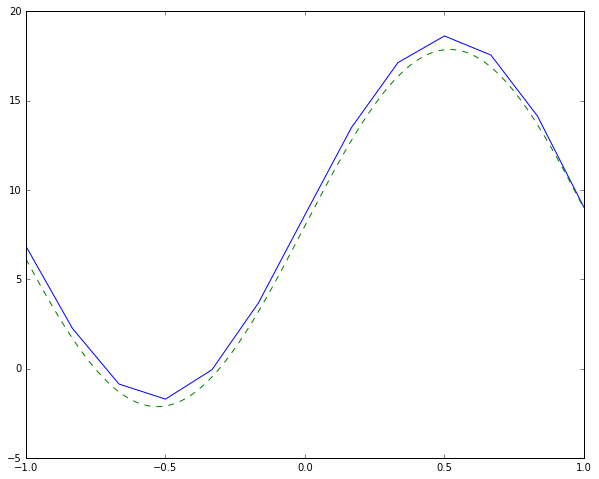
\includegraphics[width=.9\linewidth]{res1_n12}
  \caption{\it При \(n = 12\)}
  \label{fig:sub1}
\end{subfigure}%
\begin{subfigure}{.5\textwidth}
  \centering
  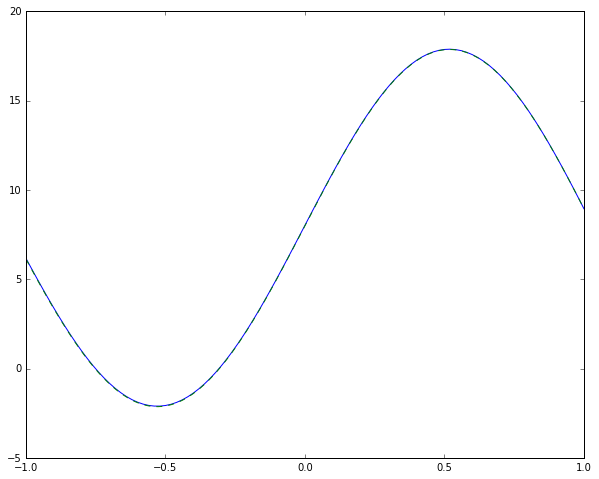
\includegraphics[width=.9\linewidth]{res1_n100}
  \caption{\it При \(n = 100\)}
  \label{fig:sub2}
\end{subfigure}
\caption{\it Результат роботи програми \cite{SourceCode} при параметрах, наведених у таблиці. Зеленим пунктиром зображено точний розв'язок, а пурпурною лінією -- чисельний розв'язок. Можна побачити, що навіть при малих значеннях \(n\), метод дає дуже гарні результати апроксимації.}
\label{fig:res1}
\end{figure}


\newpage
Наведемо приклад, де чисельний роз'язок методом безпосередньої заміни диференціальних похідних частковими не збігається до точного розв'язку.

\begin{figure}[h!]
\begin{center}
	%                  a   b   m1  m2  m3  m4  m5  k1  k2  k3  p1  p2  p3  q1  q2  q3  a1  a2
    \begin{tabular}{| l | l | l | l | l | l | l | l | l | l | l | l | l | l | l | l | l | l |}
	\hline
	a & b & $m_1$ & $m_2$ & $m_3$ & $m_4$ & $m_5$ & $k_1$ & $k_2$ & $k_3$ & $p_1$ & $p_2$ & $p_3$ & $q_1$ & $q_2$ & $q_3$ & $\alpha_1$ & $\alpha_2$ \\\hline
	$-\pi$ & $\pi$ & 10 & 3 & 1 & 1 & 7 & 2 & 2 & 1 & 4 & 1 & 1 & 1 & 2 & 1 & 1 & 1\\ \hline
    \end{tabular}
\end{center}
\bigskip
\centering
\begin{subfigure}{.5\textwidth}
  \centering
  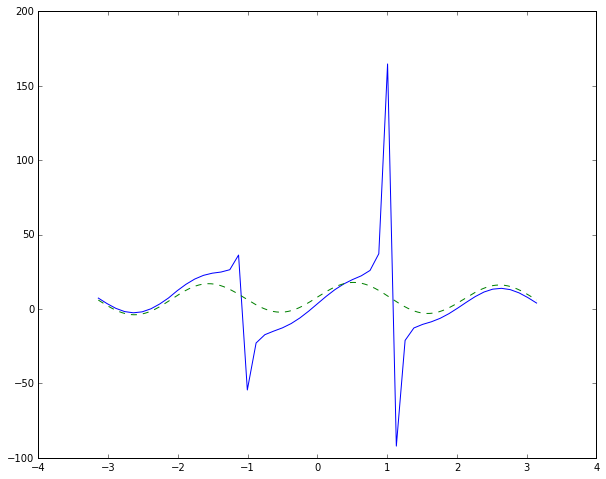
\includegraphics[width=.95\linewidth]{res2_n50}
  \caption{\it При \(n = 12\)}
  \label{fig:sub1}
\end{subfigure}%
\begin{subfigure}{.5\textwidth}
  \centering
  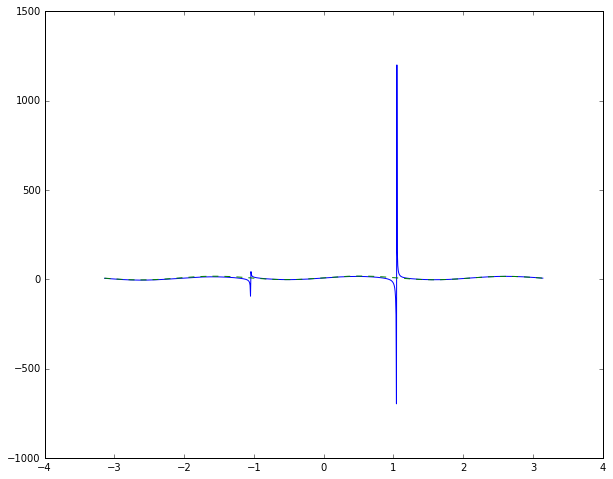
\includegraphics[width=.95\linewidth]{res2_n1500}
  \caption{\it При \(n = 100\)}
  \label{fig:sub2}
\end{subfigure}
\caption{{\it Результат роботи програми \cite{SourceCode} при параметрах, наведених у таблиці. Зеленим пунктиром зображено точний розв'язок, а пурпурною лінією -- чисельний розв'язок. Можна побачити, що у цьому випадку чим менше шаг \(h\) однорідної сітки \( \overline{\omega}_h\), тим більше похибка апроксимації.}}
\label{fig:res2}
\end{figure}

У результаті, зображеної на (мал. \ref{fig:res2}) можна побачити, що різницеві схеми (\ref{diff:full_problem}) та (\ref{diff:boundary2}) не збігається до розв'язку (\ref{anal:solution}) задачі (\ref{global:problem}). Це можна пояснити тим, що, як зазначено у пункті \ref{ssec:approx}, розв'язок збігається тільки коли \( k(x) > 0\) та \(q(x) \geq 0\). У нашому прикладі, при \( k_1 = 2\) та  \( k_3 = 1\), функція \(k\) може приймати значення менше нуля, а отже, не задовольняє умовам збіжності.

\begin{thebibliography}{9}

\bibitem{TihonovSamarskii}
  А. Н. Тихонов, А. А. Самарский,
  \emph{Об однородных разностных схемах},
  Журнал вычислительной математики и математической физики, 1961.
\bibitem{Samarskii71}
  А. А. Самарский,
  \emph{Введение в теорию разностных схем},
  Главная редакция физико-математической литературы изд-ва «Наука», 
  М., 1971. 
\bibitem{SourceCode}
  Чан Х. В., \emph{Метод безпосередньої заміни диференціальних похідних частковими на мові Python 3},
  \url{https://github.com/FalconUA/numerical-analysis/blob/master/s3-2/appointment_s3-2.ipynb}, 2017.

\end{thebibliography}
\end{document}